\documentclass{beamer}

\usepackage{tikz}
\usetikzlibrary{er}

\mode<presentation>{
	\usetheme{Madrid}
	\usecolortheme{whale}
	\setbeamercovered{transparent}
}

\title[gTrack]{{\small CS293S: Internet of Things}\\An In-Depth Analysis on Weather Data from CIMIS: Estimating Evapotranspiration (ET) Values}
\author[TheShambles]{Nazmus Saquib \and Udit Paul \and Alex Ermakov \and Santha Ramamoorthy}
\institute[CS grads, UCSB]{Graduate Students\\
Department of Computer Science\\
University of California Santa Barbara}
\titlegraphic{
\includegraphics[width=0.2\textwidth]{ucsb-logo.png}}

\AtBeginSection[]
{
  \begin{frame}<beamer>
    \frametitle{Outline}
    \tableofcontents[currentsection]
  \end{frame}
}

\begin{document}
\newcommand{\continued}{\textit{(Cntd.)}}
\newcommand{\tikzstatement}[1]{\tikz\node[draw, align=center,minimum width=12cm,minimum height=1cm,fill=blue!20, text width=12cm]{#1};}
\newcommand{\tikzproblem}[1]{\tikz\node[draw, align=center,minimum width=12cm,minimum height=1cm,fill=red!20, text width=12cm]{#1};}
\newcommand{\tikzsolution}[1]{\tikz\node[draw, align=center,minimum width=12cm,minimum height=1cm,fill=green!20, text width=12cm]{#1};}
%titlepage
\begin{frame}
\titlepage
\end{frame}

\begin{frame}
	\frametitle{Outline}
	\tableofcontents
\end{frame}

\section{Introduction}
\begin{frame}
\frametitle{Introduction: Evapotranspiration (ET)}
\begin{columns}
	\begin{column}{0.5\textwidth}
		\begin{itemize}
		\setlength\itemsep{1em}
		\item Loss of water through:\\
			\begin{enumerate}
				\setlength\itemsep{1em}
				\item Evaporation and 
				\item Transpiration
			\end{enumerate}
		\item Applications:\\
			\begin{itemize}
				\setlength\itemsep{1em}
				\item Irrigation scheduling
				\item Water resource planning, etc.
			\end{itemize}
		\end{itemize}
	\end{column}
	\begin{column}{0.5\textwidth}
		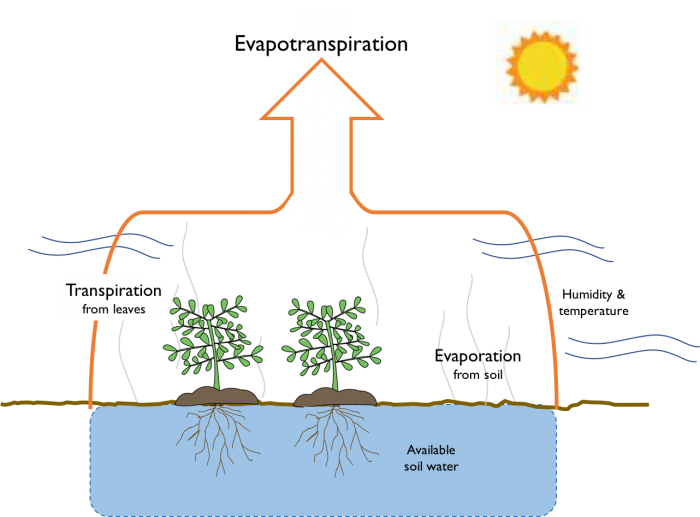
\includegraphics[width=\textwidth]{images/evapotranspiration.png}
	\end{column}
\end{columns}
\end{frame}

\begin{frame}
\frametitle{Introduction: CIMIS Weather Stations}
\begin{itemize}
\setlength\itemsep{1em}
\item \textit{California Irrigation Management Information System}
\item 257 CIMIS stations all through California\\
	\begin{itemize}
		\item 136 actively reports ET values
	\end{itemize}
\item Measures various weather parameters
\item some directly influence ET
\item Also measures (\textit{calculates?}) ET 
\end{itemize}
\end{frame}

\section{Data Collection}
\begin{frame}
\frametitle{Data Collection}
\begin{itemize}
\setlength\itemsep{1em}
\item Publicly available API
\item Reports both hourly and daily data
\item A record contains 16 different features
\item Current working dataset: data of last one year
\item Working dataset will be extended to multiple years:\\
	\begin{itemize}
	\item better for capturing seasonal variations
	\end{itemize}
\end{itemize}
\end{frame}

\section{Data Overview}
\begin{frame}
\frametitle{Sample Hourly ET Values}
\begin{figure}
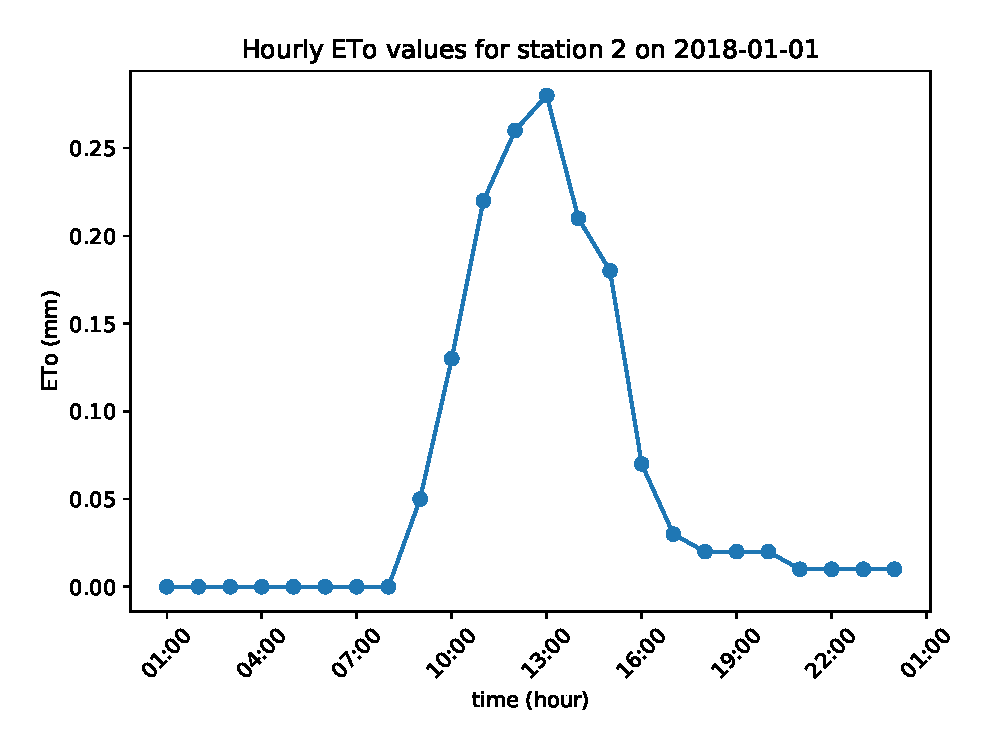
\includegraphics[width=0.9\textwidth]{images/hourly-eto-2-2018-01-01}
\end{figure}
\end{frame}

\begin{frame}
\frametitle{Mean Hourly ET Values}
\begin{figure}
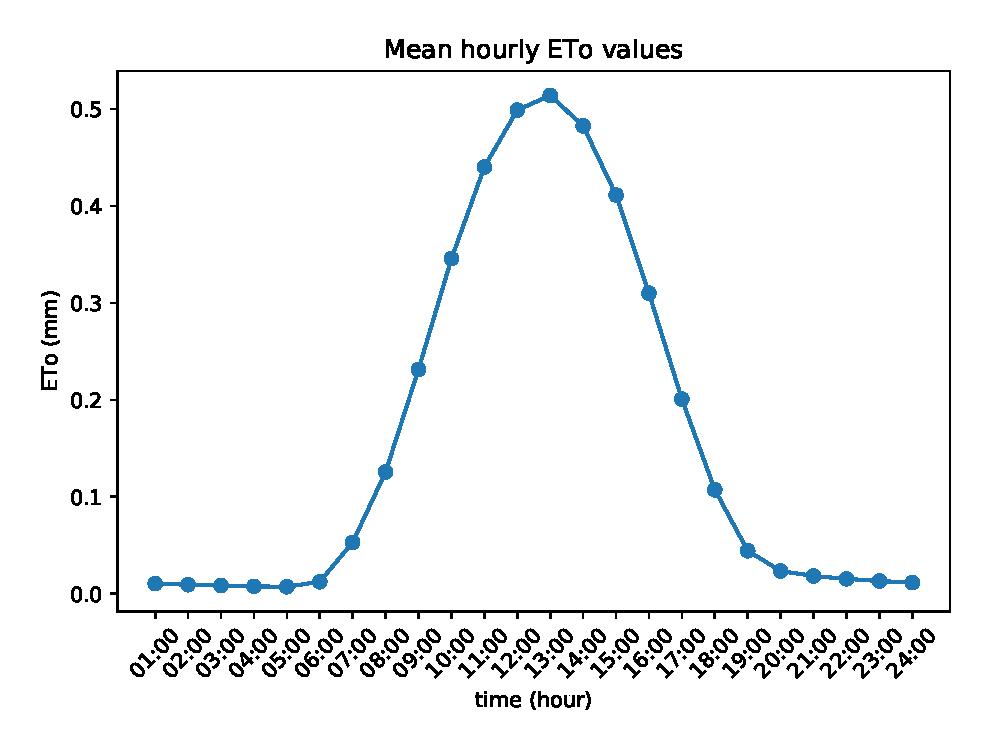
\includegraphics[width=0.9\textwidth]{images/mean-of-hourly-eto-values}
\end{figure}
\end{frame}

\begin{frame}
\frametitle{Min/Mean/Max Hourly ET Values}
\begin{figure}
	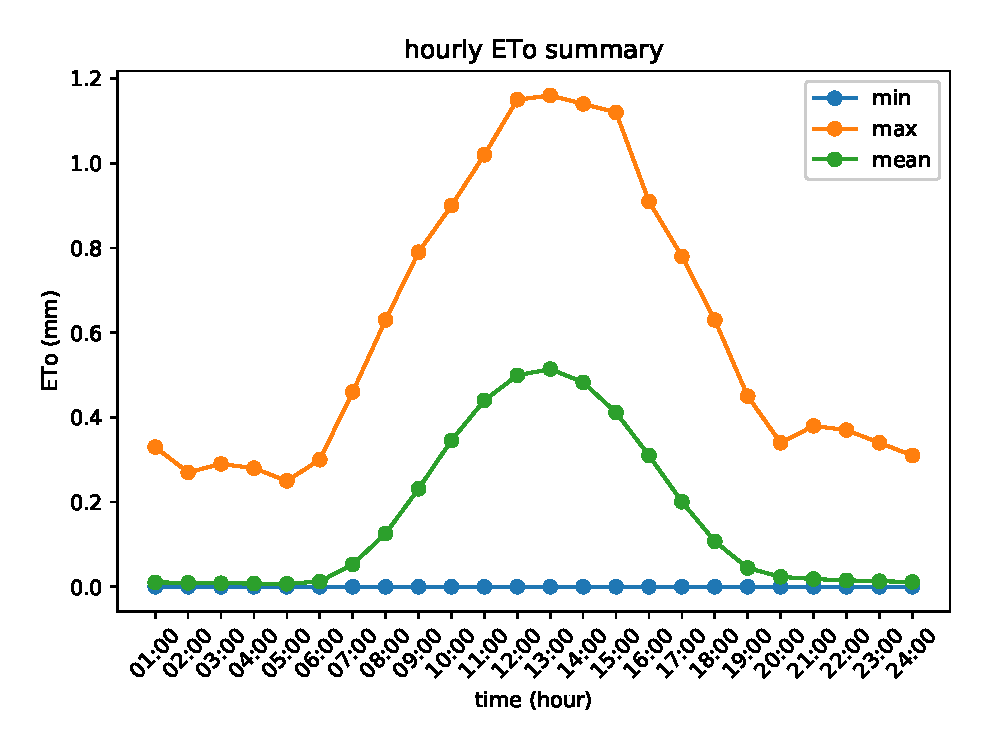
\includegraphics[width=0.9\textwidth]{images/summary-hourly-eto-values}
\end{figure}
\end{frame}

\begin{frame}
\begin{figure}
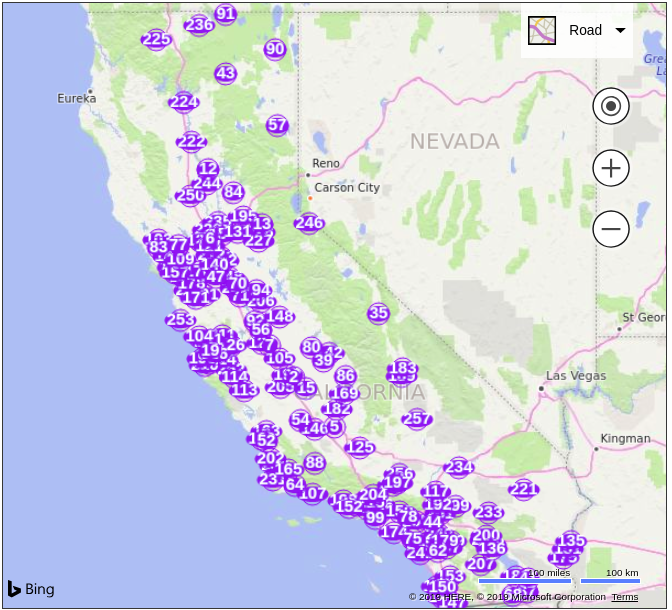
\includegraphics[width=0.8\textwidth]{images/cimis-station-location}
\end{figure}
\end{frame}

\begin{frame}
\frametitle{Stations of Interest}
\begin{itemize}
	\setlength\itemsep{1em}
	\item Station with lowest latitude $LAT_{MIN}$ (south)
	\item Station with highest latitude $LAT_{MAX}$ (north)
	\item Station with latitude closests to $\frac{LAT_{MIN}+LAT_{MAX}}{2}$ (middle)
\end{itemize}
\end{frame}

\begin{frame}
\frametitle{Mean Hourly ET Values of Stations of Interest}
\begin{figure}
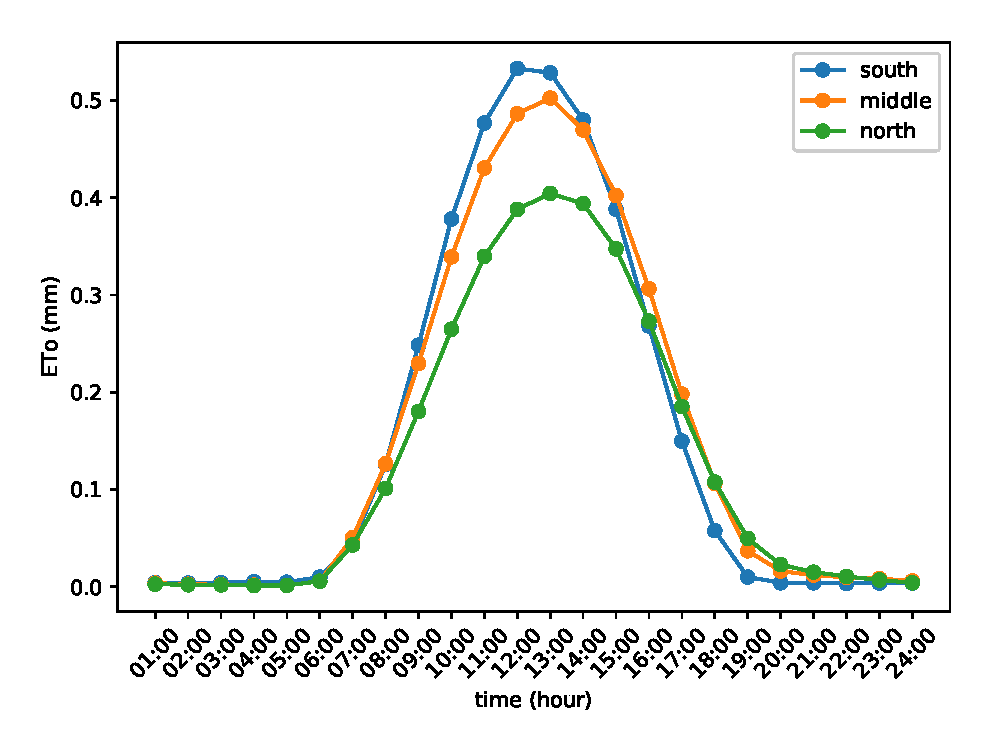
\includegraphics[width=0.9\textwidth]{images/soi-latitude-mean-of-hourly-eto-values}
\end{figure}
\end{frame}



\begin{frame}
\frametitle{Histogram of ET Values}
\begin{figure}
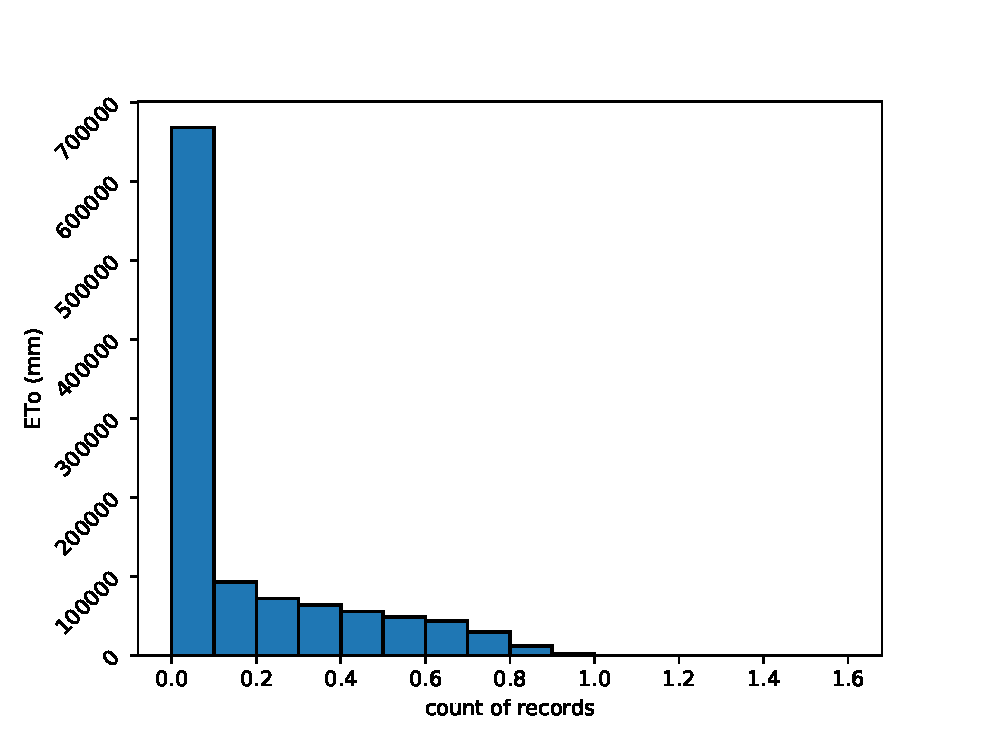
\includegraphics[width=0.9\textwidth]{images/hist-eto}
\end{figure}
\end{frame}

\begin{frame}
\frametitle{Empirical CDF of ET Values}
\begin{figure}
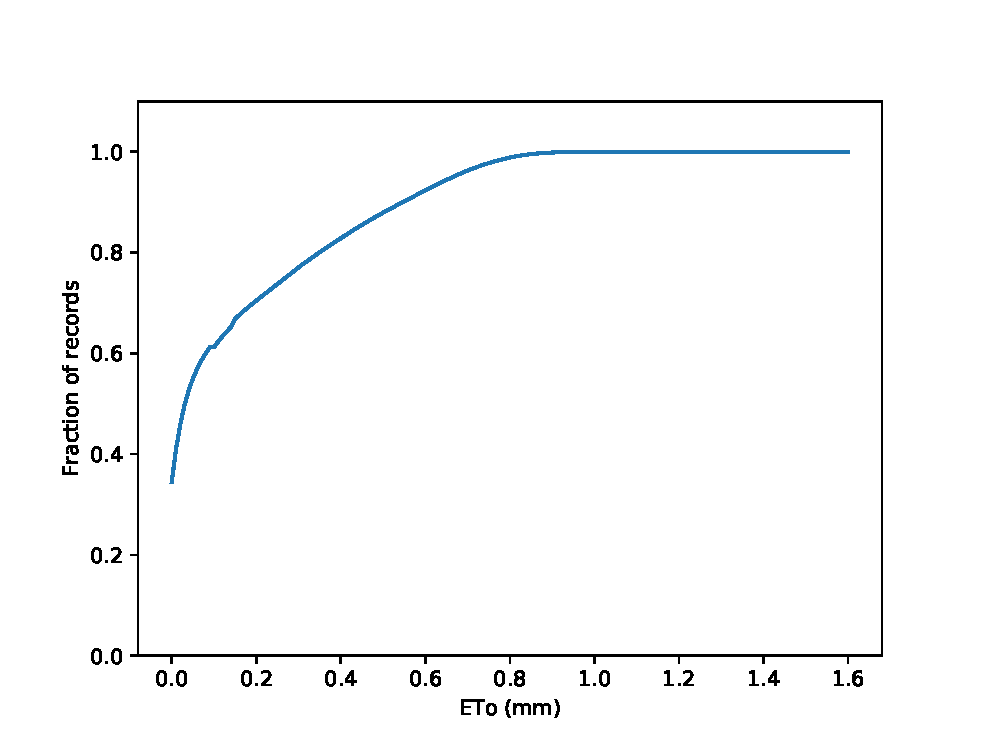
\includegraphics[width=0.9\textwidth]{images/ecdf}
\end{figure}
\end{frame}

\section{Regression Analysis}
\begin{frame}
\frametitle{Estimation of ET Values}
\tikzproblem{Given a set of features, can we estimate ET?}
\begin{itemize}
\setlength\itemsep{1em}
\item Which features to choose?
\item \textit{How well} is our estimate?
\end{itemize}
\end{frame}

\begin{frame}
\frametitle{(CIMIS) Penman Monteith Equation for Calculating ET}
\begin{equation*}
\boxed{ET_o = \frac{\bigtriangleup(R_n-G)}{\lambda[\bigtriangleup+\gamma(1+C_du_2)]} + \frac{\gamma\frac{37}{T_a+273.16}u_2(e_s-e_a)}{\bigtriangleup+\gamma(1+C_du_2)}}
\end{equation*}
\tikzstatement{Ultimately depends on four weather features}
\begin{itemize}
\setlength\itemsep{1em}
\item Solar net radiation
\item Vapor pressure
\item Air temperature
\item Wind speed
\end{itemize}
\end{frame}

\begin{frame}
\frametitle{Scatterplot Matrix of Features of Interest}
\begin{figure}
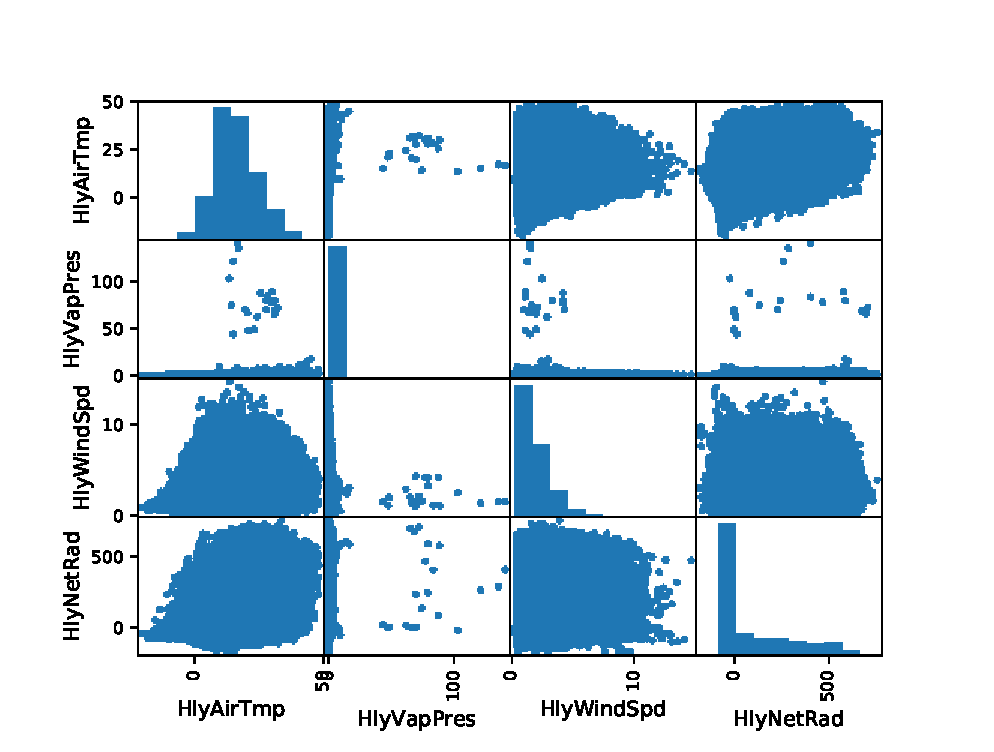
\includegraphics[width=0.85\textwidth]{images/scatterplot-matrix-HlyAirTmp-HlyVapPres-HlyWindSpd-HlyNetRad}
\end{figure}
\end{frame}

\begin{frame}
\frametitle{Regression Results}
\footnotesize
\begin{tabular}{|l|l|l|}
\hline
\textbf{Features} & \textbf{Mean Squared Error} & \textbf{$R^2$ Value}\\
\hline
HlyAirTmp,HlyNetRad,HlyVapPres,HlyWindSpd & 0.000970123960314 & 0.981294016164\\
\hline
HlyAirTmp,HlyNetRad,HlyVapPres & 0.00130358866256 & 0.974761220654\\
\hline
HlyAirTmp,HlyNetRad,HlyWindSpd & 0.00131186536214 & 0.974527982555\\
\hline
HlyAirTmp,HlyNetRad & 0.00173654973306 & 0.966537004752\\
\hline
HlyNetRad,HlyVapPres,HlyWindSpd & 0.00248645097725 & 0.952009857384\\
\hline
HlyNetRad,HlyWindSpd & 0.0024909080494 & 0.951659909255\\
\hline
HlyNetRad,HlyVapPres & 0.00302176798112 & 0.941065800356\\
\hline
HlyNetRad & 0.00304665078019 & 0.940955854127\\
\hline
HlyAirTmp,HlyVapPres,HlyWindSpd & 0.0236668111725 & 0.540318481\\
\hline
HlyAirTmp,HlyWindSpd & 0.0242823252297 & 0.528560618195\\
\hline
HlyAirTmp,HlyVapPres & 0.026563048828 & 0.485028160007\\
\hline
HlyAirTmp & 0.0278295291341 & 0.459710153733\\
\hline
HlyVapPres,HlyWindSpd & 0.0407552684279 & 0.208827525819\\
\hline
HlyWindSpd & 0.0412914020576 & 0.196118554063\\
\hline
HlyVapPres & 0.0510006461517 & 0.0128578989128\\
\hline
\end{tabular}
\end{frame}

\section{Nearest Neighbor Analysis}
\begin{frame}
\frametitle{Nearest Neighbor Analysis}
\tikzproblem{Given the ET value of $k$ nearest stations of a place, can we estimate ET?}
\begin{itemize}
\setlength\itemsep{1em}
\item Arithmetic mean of $k$ values
\item Inverse Distance Weighted (IDW) average of $k$ values
\end{itemize}
\end{frame}

\begin{frame}
\begin{figure}
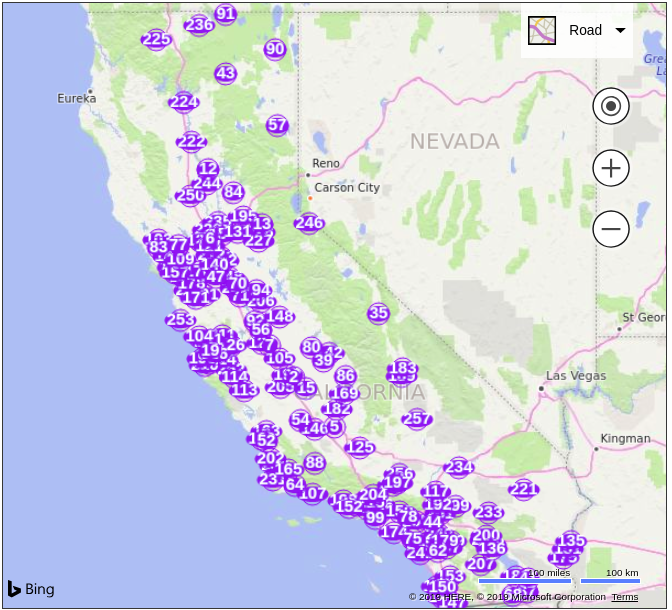
\includegraphics[width=0.8\textwidth]{images/cimis-station-location}
\end{figure}
\end{frame}

\begin{frame}
\frametitle{Stations of Interest}
\begin{itemize}
	\setlength\itemsep{1em}
	\item Station with lowest distance $D_{MIN}$ to nearest neighbor
	\item Station with highest distance $D_{MAX}$ to nearest neighbor
	\item Station with nearest neighbor at a distance closest to $\frac{D_{MIN}+D_{MAX}}{2}$
\end{itemize}
\end{frame}

\begin{frame}
\frametitle{Nearest Neighbor Results}
\centering
\footnotesize
\begin{tabular}{|l|l|l|l|}
\hline
\textbf{Station Number} & \textbf{Num of Neighbors} & \textbf{MSE for Average} &\textbf{MSE for IDW}\\
\hline
129 & 1 & 0.000832971114168 & 0.000832971114168\\
\hline
234 & 1 & 0.00437018526497 & 0.00437018526497\\
\hline
57 & 1 & 0.00451400872516 & 0.00451400872516\\
\hline
129 & 2 & 0.00116361600992 & 0.000620877927137\\
\hline
234 & 2 & 0.00761026004119 & 0.00730456269316\\
\hline
57 & 2 & 0.00371994564336 & 0.0037154634375\\
\hline
129 & 3 & 0.000890784115612 & 0.000596760525931\\
\hline
234 & 3 & 0.00908058999082 & 0.00863260116925\\
\hline
57 & 3 & 0.00335367604618 & 0.00334925237208\\
\hline
129 & 4 & 0.00116647617403 & 0.00063999172153\\
\hline
234 & 4 & 0.00919325287807 & 0.00878339044833\\
\hline
57 & 4 & 0.00361403432169 & 0.00357201358681\\
\hline
\end{tabular}
\end{frame}

\begin{frame}
\begin{figure}
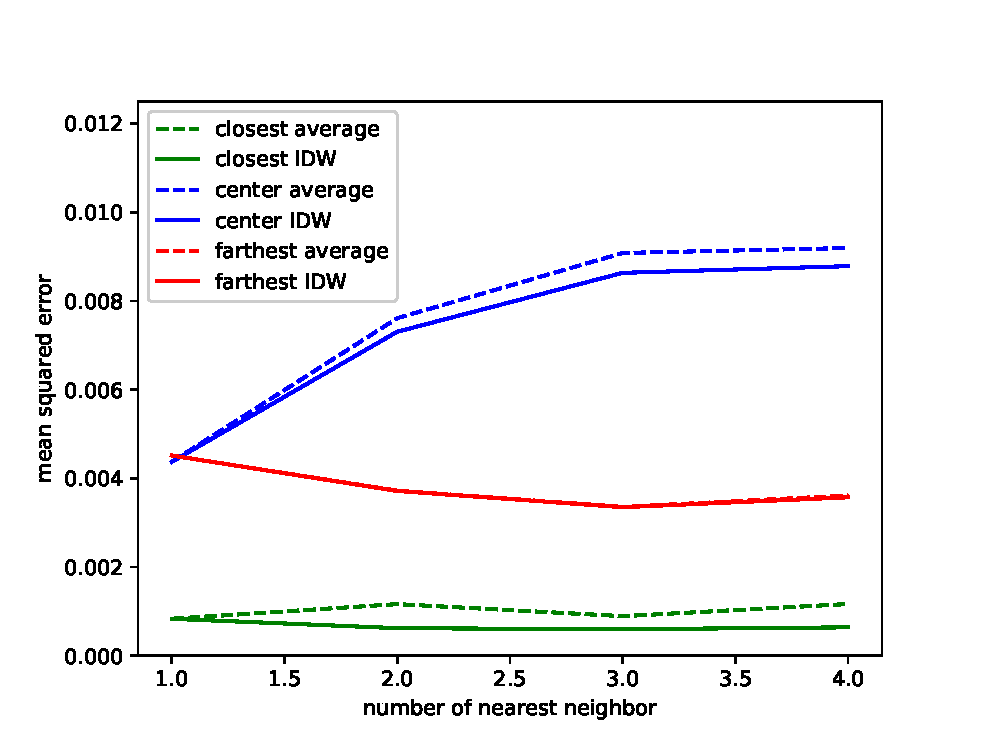
\includegraphics[width=1.0\textwidth]{images/soi-nearest-distance}
\end{figure}
\end{frame}

\begin{frame}
\frametitle{A Different Approach to Nearest Neighbor}
\begin{itemize}
\setlength\itemsep{1em}
\item Some stations are sparsely located, some are densely located
\item Distance to $n$th nearest station for different stations might vary widely
\end{itemize}
\tikzproblem{What is an optimal value of $R$ such that $k\prime$ stations\\ within that radius gives best overall estimates?}
\tikzsolution{future work $\ldots$}
\end{frame}

\section{Conclusion}
\begin{frame}
\frametitle{Future Work}
\begin{itemize}[<+->]
\setlength\itemsep{1em}
\item 4 features used in equation, do the other 12 have significant effect on ET?
\item Can the dimensionality of dataset be reduced using PCA/LDA?
\item Given one (or more, but not all) sensor value at a particular place, how well can we estimate ET by taking into account other sensor values for nearby stations?
\item Integrate web interface for analysis.
\item Cross check with ground truth value of other sources (\textit{Problem:} features seem to be different?)
\end{itemize}
\end{frame}

\section{Questions}
\begin{frame}
	\begin{center}
		{\fontsize{20}{20}\selectfont
			\textbf{Questions?}
		}
	\end{center}
\end{frame}


\end{document}
